\documentclass[a4 paper]{article}
% Set target color model to RGB
\usepackage[inner=1.5cm,outer=1.5cm,top=2.5cm,bottom=2.5cm]{geometry}
\usepackage{setspace}
\usepackage[rgb]{xcolor}
\usepackage{verbatim}
\usepackage{amsgen,amsmath,amstext,amsbsy,amsopn,tikz,amssymb,tkz-linknodes}
\usepackage{fancyhdr}
\usepackage[colorlinks=true, urlcolor=blue,  linkcolor=blue, citecolor=blue]{hyperref}
\usepackage[colorinlistoftodos]{todonotes}
\usepackage{rotating}
%\usetikzlibrary{through,backgrounds}
\hypersetup{%
pdfauthor={Arman Shokrollahi},%
pdftitle={Homework},%
pdfkeywords={Tikz,latex,bootstrap,uncertaintes},%
pdfcreator={PDFLaTeX},%
pdfproducer={PDFLaTeX},%
}
%\usetikzlibrary{shadows}
\usepackage[francais]{babel}
\usepackage{booktabs}
\newcommand{\ra}[1]{\renewcommand{\arraystretch}{#1}}

      \newtheorem{thm}{Theorem}[section]
      \newtheorem{prop}[thm]{Proposition}
      \newtheorem{lem}[thm]{Lemma}
      \newtheorem{cor}[thm]{Corollary}
      \newtheorem{defn}[thm]{Definition}
      \newtheorem{rem}[thm]{Remark}
      \numberwithin{equation}{section}

\newcommand{\homework}[6]{
   \pagestyle{myheadings}
   \thispagestyle{plain}
   \newpage
   \setcounter{page}{1}
   \noindent
   \begin{center}
   \framebox{
      \vbox{\vspace{2mm}
    \hbox to 6.28in { {\bf\hfill} }
       \vspace{6mm}
       \hbox to 6.28in { {\Large \hfill #1 (#2)  \hfill} }
       \vspace{6mm}
       \hbox to 6.28in { {\it Instructor: #3 \hfill Student: #5} }
       %\hbox to 6.28in { {\it TA: #4  \hfill #6}}
      \vspace{2mm}}
   }
   \end{center}
   \markboth{#5 -- #1}{#5 -- #1}
   \vspace*{4mm}
}

\newcommand{\bbF}{\mathbb{F}}
\newcommand{\bbX}{\mathbb{X}}
\newcommand{\bI}{\mathbf{I}}
\newcommand{\bX}{\mathbf{X}}
\newcommand{\bY}{\mathbf{Y}}
\newcommand{\bepsilon}{\boldsymbol{\epsilon}}
\newcommand{\balpha}{\boldsymbol{\alpha}}
\newcommand{\bbeta}{\boldsymbol{\beta}}
\newcommand{\0}{\mathbf{0}}

\begin{document}
\homework{Actividad \#2}{Elementos de la programaci\'on en Python 1}{Carlos Liz\'arraga Celaya}{}{Antonio Cota Rodr\'iguez}{}

\section*{Introducci\'on, ?`Qu\'e es Python?}

Python es un lenguaje de programaci\'on interpretado cuya filosof\'ia hace hincapi\'e en una sintaxis que favorezca un c\'odigo legible. Se trata de un lenguaje de programaci\'on multiparadigma, ya que soporta orientaci\'on a objetos, programaci\'on imperativa y, en menor medida, programaci\'on funcional.

\section*{Progamas}

\subsection*{Ca\'ida de una pelota}

El primer programa que se realiz\'o en esta pr\'actia fue de el {\it caida.py} el c\'odigo es el siguiente:

\begin{verbatim}

h = float(input("Proporciona la altura de la torre: "))
t = float(input("Ingresa el tiempo: "))
s = 0.5*9.81*t**2
print("La altura de la pelota es", h-s, "metros")

\end{verbatim}

Lo \'unico que se le mofidic\'o a este programa fue que se solicitar\'a expl\'icitamente al usuario la altura en metros, a continuación se muestra un ejemplo que se desarrollo en {\bf IPython Notebook}.

\vspace{0.3cm}

\begin{figure}[!ht]
  \centering
      \includegraphics[width=14.8cm, height=4.6cm]{Ca_da.png}
  \caption{Ca\'ida.py}
\end{figure}

\vspace{0.3cm}

\subsection*{Altura de un s\'atelite}

El siguiente c\'odigo es para calcular la altura de un s\'atelite en \'orbita alrededor de la tierra en funci\'on del per\'iodo (en segundos) dado por el usuario:

\begin{verbatim}

import math
G = 6.67e-11 #Constante de Gravitaci\'on universal
M = 5.97e24 #Masa de la Tierra en kilogramos
R = 6371e3 #Radio de la Tierra en metros
T = float(input("Proporciona el valor deseado para el per\'iodo de la \'orbita en segundos: "))
h = ((G*M*T**2)/(4*(math.pi)**2))**(1/3) - R
print("La altura del sat\'elite es de ", h, "metros")

\end{verbatim}

\newpage

Los siguiente ejemplos que se hicieron fue para un per\'iodo de un d\'ia y otro de 90 minutos.

\vspace{0.5cm}

\begin{figure}[!ht]
  \centering
      \includegraphics[width=14.8cm, height=4.6cm]{orbitasatelite.png}
  \caption{Per\'iodo de 1 d\'ia}
\end{figure}

\vspace{0.5cm}

\begin{figure}[!ht]
  \centering
      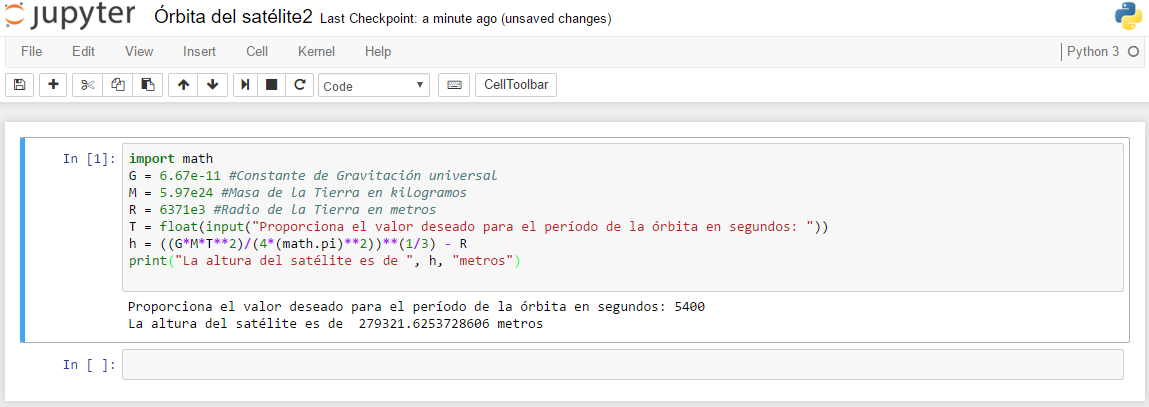
\includegraphics[width=14.8cm, height=4.6cm]{orbitasatelite2.png}
  \caption{Per\'iodo de 90 minutos}
\end{figure}

\vspace{0.5cm}

\subsection*{Transformaci\'on de coordenadas}

El siguiente c\'odigo muestra una forma de realizar una transformaci\'on de coordenadas (de cartesianas a esf\'ericas) $(x,y,z) \rightarrow (r,\theta,\phi)$:

\begin{verbatim}

from math import sin,cos,pi
r = float(input("Introduce r: "))
d = float(input("Ingresa theta en grados: "))
p = float(input("Ingresa phi en grados: "))
theta = d*pi/180
phi = d*pi/180
x = r*sin(theta)*cos(phi)
y = r*sin(theta)*sin(phi)
z = r*cos(theta)
print("x = ",x, "y =",y, "z =",z)

\end{verbatim}

\newpage

No se present\'o problema alguno, la siguiente imagen es un ejemplo con valores dados por el usuario:

\vspace{0.5cm}

\begin{figure}[!ht]
  \centering
      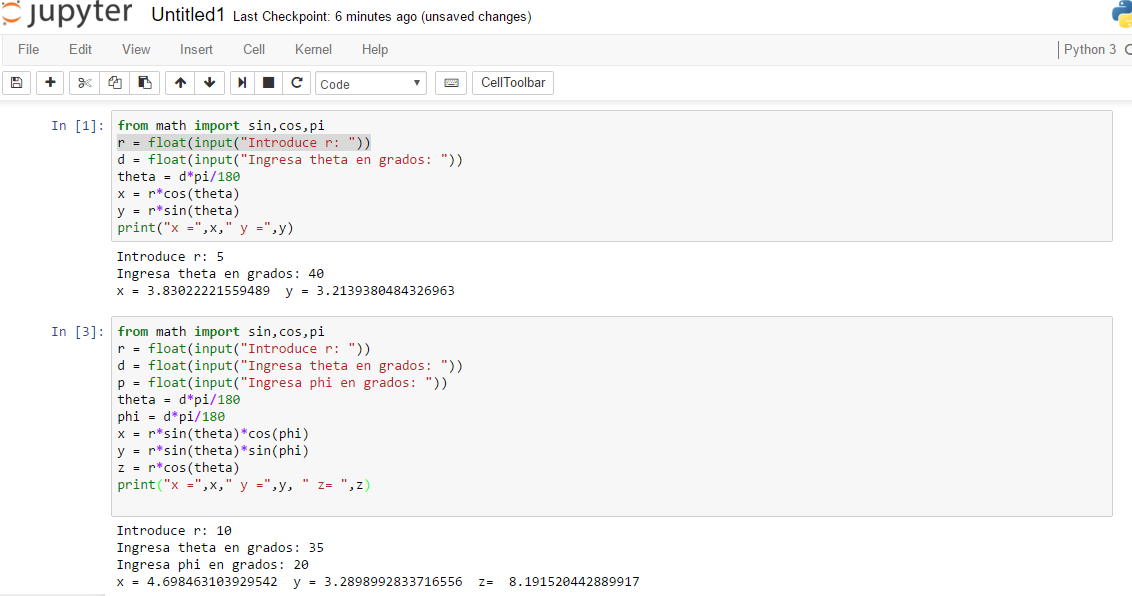
\includegraphics[width=14.8cm, height=7.75cm]{coordenadasesfericas.png}
  \caption{Ejemplo de una transformaci\'on de coordenadas}
\end{figure}

\vspace{0.5cm}

\subsection*{Par o impar}

En esta parte se cre\'o un programa en el cual se deb\'ia introducir dos valores cualesquiera enteros, el c\'odigo es el siguiente:

\begin{verbatim}
print("Enter two integers, one even, one odd.")
m = int(input("Enter the first integer: "))
n = int(input("Enter the second integer: "))
while (m+n)%2==0:
    print("One must be even and the other odd.")
    m = int(input("Enter the first integer: "))
    n = int(input("Enter the second integer: "))
print("The numbers you chose are",m,"and",n)
\end{verbatim}

Cuando el usuario introduc\'ia dos valores enteros el programa imprim\'ia una orden donde señalaba que se deb\'ian introducir un entero {\it par} y otr {\it impar} s\'olo as\'i el programa imprim\'ia los valores que se introducieron, esto debido a que en el c\'odigo escrito se espec\'ifica que el residuo debe ser diferente de cero, se muestra un ejemplo a continuaci\'on:


\begin{figure}[!ht]
  \centering
      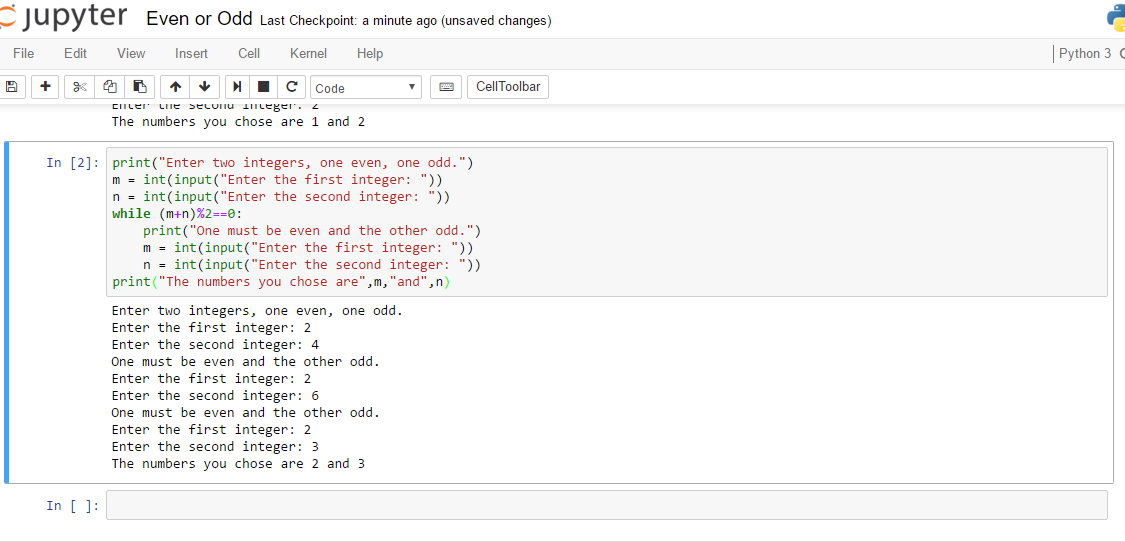
\includegraphics[width=14.8cm, height=4.75cm]{EvenOrOdd.png}
  \caption{Par o impar}
\end{figure}

\vspace{0.5cm}

\newpage

\subsection*{N\'umeros de Catal\'an}

De la misma forma que se hizo el programa de la serie de Fibonacci, esta vez se cre\'pi un programa que imprime los n\'umeros de Catal\'an menores de un millón, el c\'odigo es el siguiente

\begin{verbatim}
n,c = 0,1
while c<1000000:
      print(c)
      n,c = n+1,2*((2*n+1)/(n+2)*c)
\end{verbatim}

El resultado fue el siguiente

\vspace{0.5cm}
\begin{figure}[!ht]
  \centering
      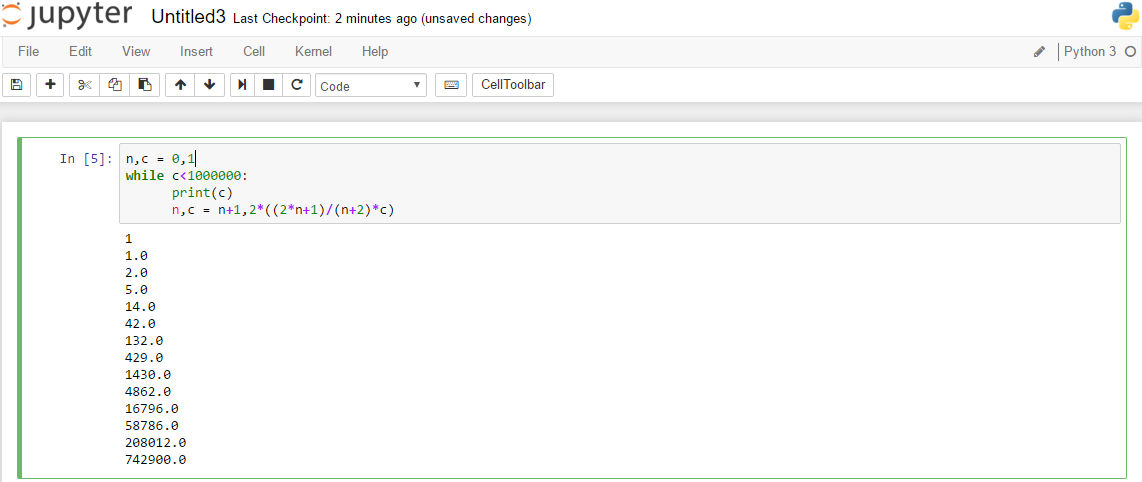
\includegraphics[width=14.8cm, height=5.75cm]{catalan.png}
  \caption{N\'umeros de Catal\'an}
\end{figure}

\vspace{0.5cm}

\end{document}

